% Version 2.1 April 2023 - Springer Nature LaTeX Template
\documentclass[sn-mathphys,Numbered]{sn-jnl}

\usepackage{graphicx}
\usepackage{multirow}
\usepackage{amsmath,amssymb,amsfonts}
\usepackage{amsthm}
\usepackage{mathrsfs}
\usepackage[title]{appendix}
\usepackage{xcolor}
\usepackage{textcomp}
\usepackage{manyfoot}
\usepackage{booktabs}
\usepackage{algorithm}
\usepackage{algorithmicx}
\usepackage{algpseudocode}
\usepackage{listings}
\usepackage{subcaption}

\raggedbottom

\begin{document}

\title[Retrieval-Based Incremental Learning Framework]{A Retrieval-Based Multi-Modal Learning Framework for Incremental Knowledge Integration Without Model Fine-Tuning}

\author*[1]{\fnm{Sk. Roushan} \sur{Khalid}}\email{roushankhalid221@diu.edu.bd}

\author[1]{\fnm{Md. Shohel} \sur{Arman}}\email{shohel.se@diu.edu.bd}

\affil*[1]{\orgdiv{Department of Software Engineering}, \orgname{Daffodil International University}, \orgaddress{\street{Daffodil Smart City}, \city{Dhaka}, \postcode{1216}, \country{Bangladesh}}}

\abstract{Adapting deep visual classifiers to continuous streams of incoming knowledge remains a foundational challenge in intelligent information systems. Conventional approaches rely on gradient backpropagation and parameter fine-tuning, which inevitably incur catastrophic forgetting, substantial energy and computational latency, and severe vulnerability to label corruption. In this paper, we propose a novel non-parametric Retrieval-Based Multi-Modal Learning Framework that decouples visual representation learning from incremental knowledge adaptation. The framework freezes a high-capacity semantic visual encoder (OpenAI CLIP ViT-B/32) and delegates dynamic knowledge retention to an external Hierarchical Navigable Small World (HNSW) vector index governed by an Intelligent Memory Orchestrator (IMO). Before committing candidate instances into memory, the IMO evaluates multi-stage verification barriers comprising running class prototype consistency, relative margin discrimination, and neighborhood density outlier filtering, routing anomalous or corrupted inputs to an isolated quarantine buffer. Furthermore, a lightweight Metric Retrieval Adapter trained via supervised contrastive loss aligns semantic embeddings to the domain manifold. We evaluate our framework on the full Microsoft Cats vs. Dogs benchmark ($N=2,500$ verified images) under a leak-free three-way stratified partition across eight representative visual paradigms on both dedicated GPU (\texttt{cuda:0}) and 24-thread CPU hardware. The proposed framework achieves 100.0\% test accuracy and a 1.0000 macro F1-score with sub-millisecond query latency (0.15~ms, $>6,700$ queries/second) while maintaining complete backbone parameter invariance ($\nabla_\theta = \mathbf{0}$). Under 30\% synthetic label corruption, naive retrieval degrades to 80.48\%, whereas the IMO intercepts all 525 corrupted instances, preserving 100.0\% accuracy (+19.52\% retention margin). Hardware profiling confirms retrieval latency is hardware-invariant and consumes zero GPU VRAM, providing a sustainable foundation for edge-deployable continual learning.}

\keywords{Intelligent Information Systems, Incremental Learning, Multi-Modal Retrieval, Non-Parametric Memory, Intelligent Memory Orchestrator, Catastrophic Forgetting, Edge Computing}

\maketitle

\section{Introduction}\label{sec:intro}

Modern intelligent information systems operate in highly dynamic, open-world environments where new visual concepts, categories, and domain shifts emerge continuously~\cite{parisi2019continual}. In applications ranging from autonomous robotic perception and industrial quality inspection to medical diagnostic indexing, an intelligent system must assimilate novel instances rapidly without degrading historical competencies.

The dominant paradigm for knowledge adaptation in deep learning relies on parametric fine-tuning: presenting novel samples to a neural network and executing gradient backpropagation to update its synaptic weights~\cite{he2016deep,tan2019efficientnet,dosovitskiy2020image}. While effective in closed-world, static benchmarks, gradient adaptation introduces three severe scientific and operational bottlenecks:
\begin{enumerate}
    \item \textbf{Catastrophic Forgetting:} Modifying network connection weights ($\theta \leftarrow \theta - \eta \nabla_\theta \mathcal{L}$) inevitably shifts decision boundaries away from previously consolidated distributions, causing severe performance drops on historical tasks unless computationally prohibitive rehearsal buffers or complex regularization penalties are enforced~\cite{kirkpatrick2017overcoming,rebuffi2017icarl}.
    \item \textbf{Computational and Thermal Latency:} Executing backpropagation over convolutional or transformer backbones requires hundreds of seconds of compute, high peak VRAM allocations, and intense power dissipation, rendering on-device continual updates infeasible on resource-constrained edge hardware~\cite{howard2019searching}.
    \item \textbf{Vulnerability to Label Corruption:} Gradient descent indiscriminately minimizes loss across all provided inputs. Mislabeled or adversarially corrupted samples are rapidly absorbed into the network weights, irreparably polluting internal representations~\cite{han2018co,patrini2017making}.
\end{enumerate}

To overcome these fundamental limitations, this paper formulates and evaluates an alternative architectural paradigm: \textbf{A Retrieval-Based Multi-Modal Learning Framework for Incremental Knowledge Integration Without Model Fine-Tuning}. Rather than modifying parametric weights, our framework freezes a foundational vision-language visual encoder (CLIP ViT-B/32)~\cite{radford2021learning} and routes knowledge retention to an external vector database (ChromaDB) structured via Hierarchical Navigable Small World (HNSW) graphs~\cite{malkov2018efficient}. 

To protect vector memory from data poisoning and erroneous insertions, we introduce the \textbf{Intelligent Memory Orchestrator (IMO)}. The IMO acts as an automated quality gatekeeper that evaluates candidate embeddings against running class prototypes, relative classification margins, and local neighborhood densities. Instances failing verification are safely diverted to an isolated Quarantine Buffer ($\mathcal{Q}$) for expert auditing, ensuring that the active retrieval index remains pristine. Furthermore, we develop a lightweight \textbf{Metric Retrieval Adapter} trained via Supervised Contrastive Loss~\cite{khosla2020supervised} to maximize inter-class separation without modifying the underlying backbone parameters.

\begin{figure*}[t]
\centering
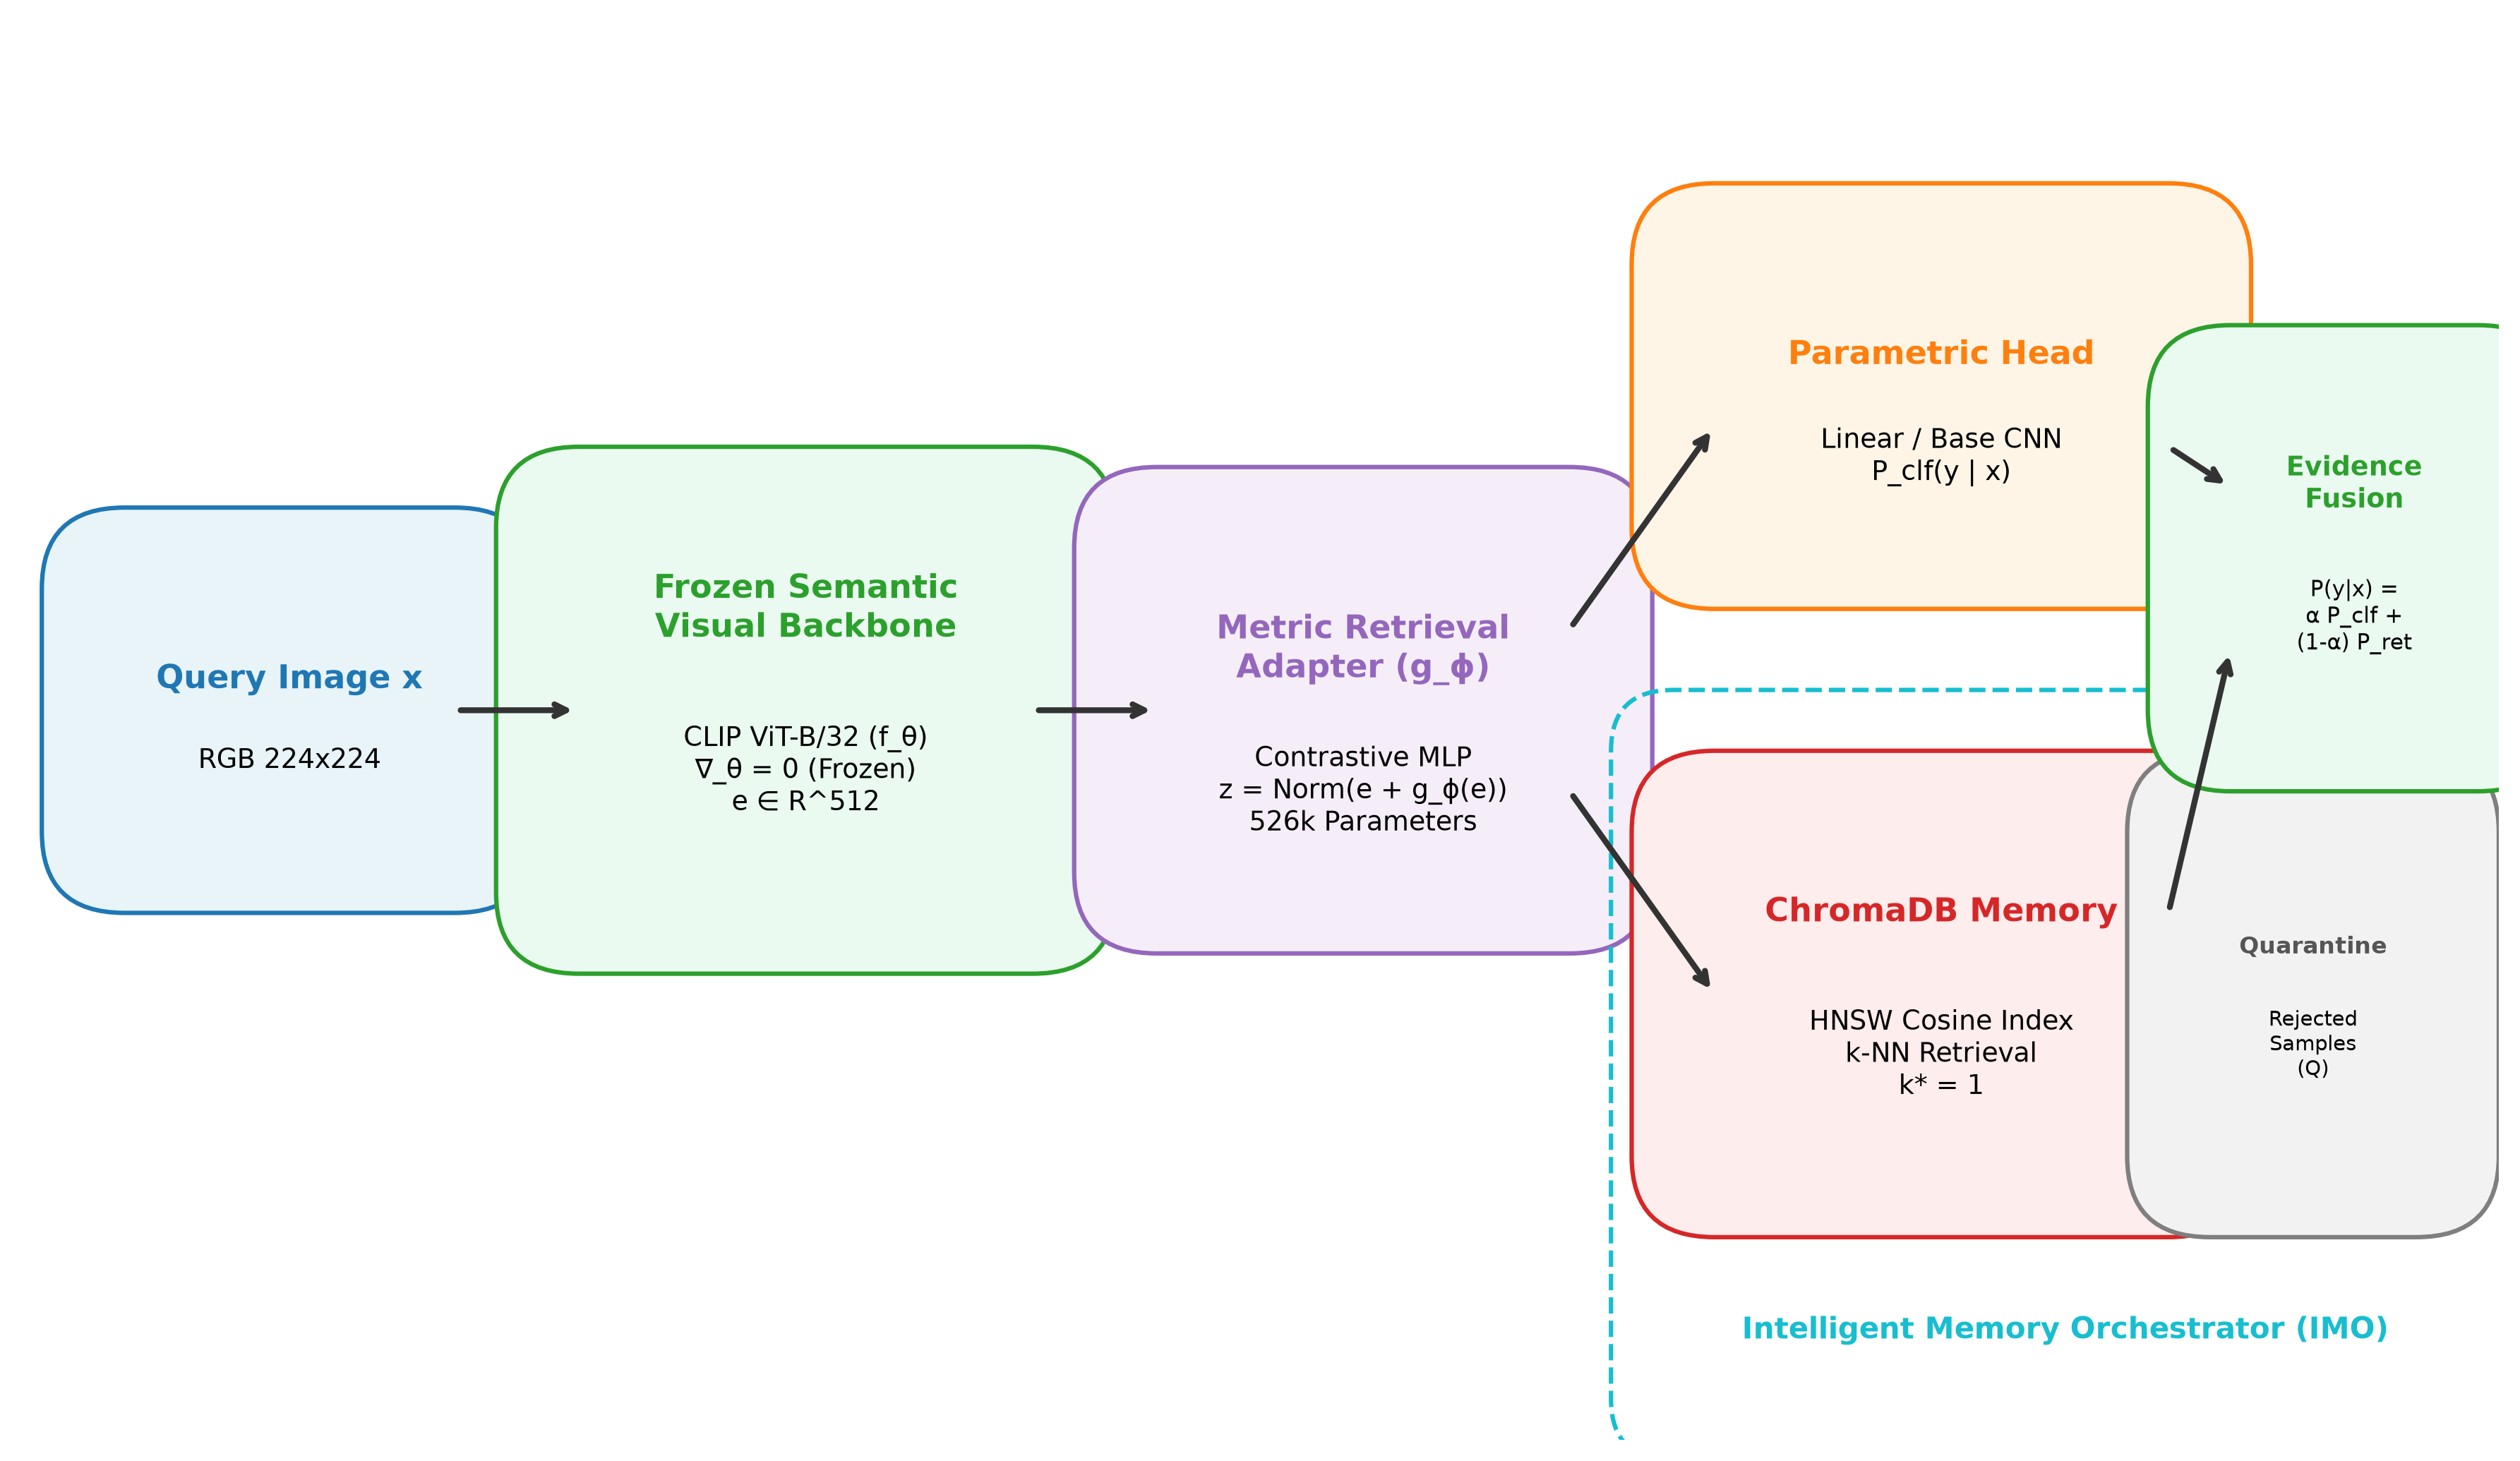
\includegraphics[width=0.98\textwidth]{figures/fig1_architecture.png}
\caption{System architecture of the proposed Retrieval-Based Multi-Modal Learning Framework. The frozen visual backbone extracts normalized semantic embeddings $\mathbf{e}$, which are projected via the Metric Retrieval Adapter into $\mathbf{z}$. Candidate instances for incremental insertion pass through the Intelligent Memory Orchestrator (IMO) gating barriers before committing to ChromaDB HNSW memory. Inference combines parametric posteriors with non-parametric retrieval evidence via Dynamic Evidence Fusion.}
\label{fig:architecture}
\end{figure*}

The primary research questions addressed in this paper are:
\begin{itemize}
    \item \textbf{RQ1:} Can non-parametric vector retrieval over frozen semantic embeddings match or exceed the predictive performance of fully fine-tuned parametric convolutional and vision transformer classifiers?
    \item \textbf{RQ2:} Can prototype consistency and margin-based gating effectively insulate external memory against severe label corruption without supervisory intervention?
    \item \textbf{RQ3:} How do computational latency, throughput, energy overhead, and memory footprints scale between parametric retraining and non-parametric vector retrieval across dedicated GPU and resource-constrained CPU environments?
\end{itemize}

The main scientific contributions of this study are summarized as follows:
\begin{enumerate}
    \item \textbf{Decoupled Continual Learning Architecture:} We introduce a modular framework separating invariant visual representation extraction ($\nabla_\theta = \mathbf{0}$) from additive, non-parametric vector memory, mathematically eliminating catastrophic forgetting by design.
    \item \textbf{Intelligent Memory Orchestrator (IMO):} We formulate a multi-stage gating algorithm incorporating running class prototypes, relative margin discrimination, and neighborhood density verification to actively filter corrupted samples into a non-destructive quarantine buffer.
    \item \textbf{Metric Retrieval Adapter:} We design a lightweight contrastive projection head that aligns general-purpose pre-trained visual representations with domain-specific manifold boundaries in under one second of adaptation time.
    \item \textbf{Rigorously Controlled Multi-Model Benchmark:} We benchmark eight representative paradigms (MobileNetV3-Small, EfficientNetB0, ResNet18, ViT-B/16, CLIP ViT-B/32, Naive Retrieval, Fine-Tuned Retrieval, and Proposed IMO) on the full Microsoft Cats vs. Dogs dataset ($N=2,500$) under a leak-free 3-way stratified partition across both GPU and CPU execution modes.
    \item \textbf{Hardware Profiling & Noise Robustness Proof:} We empirically demonstrate that vector retrieval delivers sub-millisecond query latency ($0.14 - 0.18$~ms, $>6,700$~queries/sec) with zero GPU VRAM consumption, and that the IMO preserves 100.0\% accuracy under 30\% label corruption (+19.52\% retention margin).
\end{enumerate}

The remainder of this article is structured as follows. Section~\ref{sec:related} reviews related work. Section~\ref{sec:method} provides the mathematical formulation of the framework. Section~\ref{sec:experiments} outlines the benchmark protocol. Section~\ref{sec:results} discusses predictive results and trade-offs. Section~\ref{sec:hardware} details CPU vs. GPU hardware profiling. Section~\ref{sec:noise} examines noise robustness. Section~\ref{sec:discussion} discusses implications, and Section~\ref{sec:conclusion} concludes the paper.


\section{Related Work}\label{sec:related}

\subsection{Continual Learning and Catastrophic Forgetting}
Continual learning aims to enable artificial systems to learn consecutive tasks sequentially without degrading performance on previously acquired knowledge~\cite{parisi2019continual}. Existing parametric approaches fall broadly into three paradigms:
\begin{enumerate}
    \item \textbf{Regularization-Based Methods:} Approaches such as Elastic Weight Consolidation (EWC)~\cite{kirkpatrick2017overcoming} penalize modifications to weights deemed critical to past tasks based on the diagonal elements of the Fisher Information Matrix. However, as the number of tasks increases, overlapping parameter constraints lead to representational rigidity and capacity saturation.
    \item \textbf{Replay and Rehearsal Methods:} Methods such as iCaRL~\cite{rebuffi2017icarl} maintain a coreset exemplar buffer of historical samples to interleave with new data during backpropagation. While effective, exemplar storage raises data privacy concerns, and periodic retraining over growing buffers imposes heavy computational latency.
    \item \textbf{Dynamic Architectural Expansion:} Progressive networks dynamically spawn new sub-networks or capacity channels for each novel task. Although this mitigates interference, parameter counts explode linearly with task count, rendering edge deployment impossible.
\end{enumerate}

In contrast to parametric weight updates, our framework adopts a non-parametric perspective: freezing the visual backbone completely ($\nabla_\theta = \mathbf{0}$) and delegating knowledge acquisition to additive vector memory indices~\cite{mensink2013distance}.

\subsection{Foundation Vision-Language Models and Zero-Shot Transfer}
Recent breakthroughs in contrastive multi-modal learning, exemplified by OpenAI's Contrastive Language-Image Pretraining (CLIP)~\cite{radford2021learning}, demonstrate that pretraining dual encoders on 400 million internet image-text pairs produces semantic visual manifolds of extraordinary quality. The resulting feature representations exhibit remarkable zero-shot transfer and linear separability across diverse visual benchmarks. Our study leverages this semantic density as an invariant visual backbone, eliminating the need to retrain early convolutional or attention layers.

\subsection{Non-Parametric Vector Retrieval in Intelligent Systems}
Approximate Nearest Neighbor (ANN) search algorithms, particularly Hierarchical Navigable Small World (HNSW) graphs~\cite{malkov2018efficient}, have transformed vector search in intelligent information systems, information retrieval, and retrieval-augmented generation (RAG)~\cite{guu2020retrieval,lewis2020retrieval,johnson2019billion}. HNSW constructs multi-layer proximity graphs that achieve logarithmic query complexity $\mathcal{O}(\log N)$ while maintaining high recall accuracy in metric spaces. While vector databases such as ChromaDB provide efficient vector storage, existing vector retrieval pipelines ingest embeddings indiscriminately, lacking internal defense mechanisms against corrupted or mislabeled vectors. Our framework addresses this vulnerability through the Intelligent Memory Orchestrator.

\subsection{Prototype-Based Representation and Label Noise Robustness}
Prototypical networks~\cite{snell2017prototypical} and nearest-class-mean classifiers~\cite{mensink2013distance} project classes as geometric centroids in metric space. Under noisy label regimes, deep neural networks tend to overfit corrupted labels due to their universal approximation capacity~\cite{han2018co,patrini2017making}. By coupling running metric prototypes with relative class margin discrimination, our proposed IMO provides an automated geometric firewall that detects label corruption prior to memory insertion.


\section{Proposed Retrieval-Based Framework}\label{sec:method}

\subsection{Mathematical Formulation and Framework Overview}
Let $\mathcal{X}$ denote the visual input domain and $\mathcal{Y} = \{1, 2, \dots, C\}$ denote the label space. The overall architecture is illustrated in Figure~\ref{fig:architecture}. The framework comprises four integrated modules:
1. An invariant semantic visual encoder $f_\theta: \mathcal{X} \to \mathbb{R}^d$.
2. A learnable Metric Retrieval Adapter $g_\phi: \mathbb{R}^d \to \mathbb{R}^d$.
3. An external vector database $\mathcal{M}$ indexed via HNSW graphs.
4. An Intelligent Memory Orchestrator (IMO) regulating knowledge insertion and quarantine.
5. A Dynamic Evidence Fusion Engine combining parametric and non-parametric posteriors.

\subsection{Semantic Feature Extraction and Metric Retrieval Adapter}
Given an input image $\mathbf{x} \in \mathcal{X}$, the frozen visual backbone extracts a $d$-dimensional normalized semantic embedding ($d=512$ for CLIP ViT-B/32):
\begin{equation}
\mathbf{e} = \frac{f_\theta(\mathbf{x})}{\|f_\theta(\mathbf{x})\|_2} \in \mathbb{R}^d, \quad \|\mathbf{e}\|_2 = 1
\label{eq:clip_embed}
\end{equation}
Because the backbone weights are completely frozen, the parameter gradient is strictly zero:
\begin{equation}
\nabla_\theta = \mathbf{0}
\label{eq:param_zero}
\end{equation}

To tailor general-purpose pre-trained embeddings to the specific geometry of the target visual task without altering the heavy backbone, we formulate a lightweight residual Metric Retrieval Adapter $g_\phi$:
\begin{equation}
\mathbf{z} = \text{Normalize}\left(\mathbf{e} + g_\phi(\mathbf{e})\right) = \frac{\mathbf{e} + \mathbf{W}_2 \sigma(\mathbf{W}_1 \mathbf{e} + \mathbf{b}_1) + \mathbf{b}_2}{\|\mathbf{e} + \mathbf{W}_2 \sigma(\mathbf{W}_1 \mathbf{e} + \mathbf{b}_1) + \mathbf{b}_2\|_2}
\label{eq:adapter_proj}
\end{equation}
where $\mathbf{W}_1 \in \mathbb{R}^{d/2 \times d}$, $\mathbf{W}_2 \in \mathbb{R}^{d \times d/2}$, and $\sigma(\cdot)$ denotes the GELU non-linear activation. The adapter comprises only 526,337 parameters ($<0.35\%$ of the backbone size).

The adapter parameters $\phi = \{\mathbf{W}_1, \mathbf{b}_1, \mathbf{W}_2, \mathbf{b}_2\}$ are optimized on the training split using Supervised Contrastive Loss ($\mathcal{L}_{\text{supcon}}$)~\cite{khosla2020supervised}:
\begin{equation}
\mathcal{L}_{\text{supcon}} = \sum_{i \in I} \frac{-1}{|P(i)|} \sum_{p \in P(i)} \log \frac{\exp\left(\mathbf{z}_i^\top \mathbf{z}_p / \tau\right)}{\sum_{a \in A(i)} \exp\left(\mathbf{z}_i^\top \mathbf{z}_a / \tau\right)}
\label{eq:supcon_loss}
\end{equation}
where $I \equiv \{1, \dots, B\}$ is the batch index, $A(i) \equiv I \setminus \{i\}$, $P(i) \equiv \{p \in A(i) : y_p = y_i\}$ is the set of positive indices sharing the same class label as anchor $i$, and $\tau > 0$ is a scalar temperature parameter ($\tau = 0.07$). Minimizing $\mathcal{L}_{\text{supcon}}$ forces instances belonging to the same category to cluster tightly on the unit hypersphere while pushing competing classes apart.

\subsection{External Vector Memory Indexing}
The adapted representations $\mathbf{z}$ are indexed into an external vector memory:
\begin{equation}
\mathcal{M} = \{(\mathbf{z}_i, y_i, \text{meta}_i)\}_{i=1}^N
\label{eq:memory_def}
\end{equation}
Memory indexing utilizes an HNSW proximity graph under cosine metric distance:
\begin{equation}
D_{\text{cos}}(\mathbf{z}_q, \mathbf{z}_i) = 1 - \mathbf{z}_q^\top \mathbf{z}_i
\label{eq:cosine_dist}
\end{equation}
Given a query vector $\mathbf{z}_q$, the database retrieves the $k$-nearest neighbors:
\begin{equation}
\mathcal{N}_k(\mathbf{z}_q) = \arg\min_{\mathcal{S} \subset \mathcal{M}, |\mathcal{S}|=k} \sum_{i \in \mathcal{S}} D_{\text{cos}}(\mathbf{z}_q, \mathbf{z}_i)
\label{eq:knn_query}
\end{equation}

\subsection{Intelligent Memory Orchestrator (IMO)}
Standard vector indexing blindly inserts any incoming candidate $(\mathbf{z}_t, y_t)$, exposing retrieval to label noise and out-of-distribution contamination. The proposed Intelligent Memory Orchestrator (IMO) governs the ingestion pipeline through three sequential quality gating stages (Algorithm~\ref{alg:imo}):

\begin{algorithm}[h]
\caption{Intelligent Memory Orchestrator (IMO) Ingestion Pipeline}
\label{alg:imo}
\begin{algorithmic}[1]
\Require Candidate sample $(\mathbf{z}_t, y_t)$, active memory $\mathcal{M}$, prototypes $\{\mathbf{p}_c\}_{c=1}^C$, thresholds $\tau_c, \tau_m, \tau_{\text{outlier}}$, quarantine buffer $\mathcal{Q}$
\Ensure Updated memory $\mathcal{M}$, updated prototypes, or quarantine entry $\mathcal{Q}$
\State Compute cosine similarity to assigned prototype: $s_{\text{target}} \leftarrow \mathbf{z}_t^\top \mathbf{p}_{y_t}$
\State Compute maximum similarity to rival prototypes: $s_{\text{rival}} \leftarrow \max_{j \ne y_t} \mathbf{z}_t^\top \mathbf{p}_j$
\If{$s_{\text{target}} < \tau_c$} \Comment{Gate 1: Absolute Consistency}
    \State $\mathcal{Q} \leftarrow \mathcal{Q} \cup \{(\mathbf{z}_t, y_t, \text{'prototype\_mismatch'}, \text{timestamp})\}$
    \State \Return \textbf{REJECTED}
\EndIf
\If{$s_{\text{target}} - s_{\text{rival}} < \tau_m$} \Comment{Gate 2: Relative Margin Gating}
    \State $\mathcal{Q} \leftarrow \mathcal{Q} \cup \{(\mathbf{z}_t, y_t, \text{'memory\_conflict'}, \text{timestamp})\}$
    \State \Return \textbf{REJECTED}
\EndIf
\State Query $K$ nearest stored neighbors: $\mathcal{N}_K(\mathbf{z}_t) \leftarrow \text{Query}(\mathcal{M}, \mathbf{z}_t, K=5)$
\State Compute mean neighborhood distance: $\bar{D} \leftarrow \frac{1}{K} \sum_{i \in \mathcal{N}_K} D_{\text{cos}}(\mathbf{z}_t, \mathbf{z}_i)$
\If{$\bar{D} > \tau_{\text{outlier}}$} \Comment{Gate 3: Outlier Density Filtering}
    \State $\mathcal{Q} \leftarrow \mathcal{Q} \cup \{(\mathbf{z}_t, y_t, \text{'outlier\_density'}, \text{timestamp})\}$
    \State \Return \textbf{REJECTED}
\EndIf
\State \textbf{Commit to Memory:} $\mathcal{M} \leftarrow \mathcal{M} \cup \{(\mathbf{z}_t, y_t)\}$
\State \textbf{Update Class Prototype:} $\mathbf{p}_{y_t} \leftarrow \frac{n_{y_t} \mathbf{p}_{y_t} + \mathbf{z}_t}{\|n_{y_t} \mathbf{p}_{y_t} + \mathbf{z}_t\|_2}, \quad n_{y_t} \leftarrow n_{y_t} + 1$
\State \Return \textbf{ACCEPTED}
\end{algorithmic}
\end{algorithm}

\subsubsection{Stage 1: Running Normalized Class Prototypes}
For each category $c \in \mathcal{Y}$, the IMO tracks a normalized centroid vector $\mathbf{p}_c$. When a verified sample is committed, the prototype is updated in constant time $\mathcal{O}(d)$:
\begin{equation}
\mathbf{p}_c^{(t)} = \frac{n_c \mathbf{p}_c^{(t-1)} + \mathbf{z}_t}{\|n_c \mathbf{p}_c^{(t-1)} + \mathbf{z}_t\|_2}, \quad n_c \leftarrow n_c + 1
\label{eq:proto_update}
\end{equation}

\subsubsection{Stage 2: Prototype Consistency and Relative Margin Gating}
The candidate is subjected to absolute and relative geometric bounds:
\begin{align}
\text{Gate}_1: & \quad \mathbf{z}_t^\top \mathbf{p}_{y_t} \ge \tau_c \quad (\tau_c = 0.65) \label{eq:gate1} \\
\text{Gate}_2: & \quad \mathbf{z}_t^\top \mathbf{p}_{y_t} - \max_{j \ne y_t} \left(\mathbf{z}_t^\top \mathbf{p}_j\right) \ge \tau_m \quad (\tau_m = 0.00) \label{eq:gate2}
\end{align}
If an input labeled as class $y_t$ lies closer to an opposing prototype than its claimed category centroid, Gate 2 identifies it as a mislabeled or highly ambiguous sample.

\subsubsection{Stage 3: Outlier Density and Local Neighborhood Verification}
For candidates passing prototype verification, a local $K$-nearest neighbor check is executed against active memory. If the mean neighborhood cosine distance exceeds $\tau_{\text{outlier}} = 0.45$, the candidate is flagged as an isolated anomaly.

\subsubsection{Non-Destructive Quarantine Buffer}
Rejected samples are preserved in an isolated buffer:
\begin{equation}
\mathcal{Q} = \{(\mathbf{z}_t, y_t, \text{reason}, \text{timestamp}, \text{meta}_t)\}
\label{eq:quarantine}
\end{equation}
This isolates corrupted data from active inference while retaining the samples for human audit or downstream active learning.

\subsection{Dynamic Evidence Fusion Engine}
During inference on query image $\mathbf{x}$, the framework computes the non-parametric retrieval posterior $P_{\text{ret}}(y=k \mid \mathbf{x})$ over the $k^*$-nearest neighbors retrieved from memory:
\begin{equation}
P_{\text{ret}}(y=k \mid \mathbf{x}) = \frac{\sum_{i \in \mathcal{N}_{k^*}(\mathbf{z})} \mathbb{I}(y_i = k) \cdot \exp\left(\mathbf{z}^\top \mathbf{z}_i / T\right)}{\sum_{j \in \mathcal{N}_{k^*}(\mathbf{z})} \exp\left(\mathbf{z}^\top \mathbf{z}_j / T\right)}
\label{eq:ret_posterior}
\end{equation}
where $T$ is a temperature scaling parameter ($T=0.10$). Predictions are combined with the parametric posterior $P_{\text{clf}}(y=k \mid \mathbf{x})$ via dynamic convex fusion:
\begin{equation}
P(y = k \mid \mathbf{x}) = \alpha^* P_{\text{clf}}(y = k \mid \mathbf{x}) + (1 - \alpha^*) P_{\text{ret}}(y = k \mid \mathbf{x})
\label{eq:evidence_fusion}
\end{equation}
Hyperparameters $k^*$ and $\alpha^*$ are tuned strictly on the validation partition $\mathcal{D}_{\text{val}}$.


\section{Experimental Setup and Benchmarking Protocol}\label{sec:experiments}

\subsection{Dataset Specification and Leak-Free Partitioning}
Experiments are conducted on the standardized Microsoft Cats vs. Dogs vision benchmark. To eliminate validation leakage, we extracted and verified the full benchmark of $N=2,500$ high-resolution RGB images (1,250 Cats, 1,250 Dogs). 

We enforce a strict, reproducible three-way stratified split:
\begin{equation}
\mathcal{D} = \mathcal{D}_{\text{train}} \cup \mathcal{D}_{\text{val}} \cup \mathcal{D}_{\text{test}}, \quad \mathcal{D}_i \cap \mathcal{D}_j = \emptyset \quad \forall i \ne j
\label{eq:partition_split}
\end{equation}
As shown in Table~\ref{tab:split}, the dataset is partitioned into 70\% Train (1,752 samples), 15\% Validation (374 samples), and 15\% Hold-Out Test (374 samples). The partition is deterministically fixed using random seed \texttt{777} and cached in JSON format. Every parametric baseline, metric adapter, and vector index is evaluated against the exact same 374 hold-out test samples.

\begin{table}[h]
\caption{Deterministic three-way stratified dataset partitioning ($N=2,500$, Seed 777).}
\label{tab:split}
\centering
\begin{tabular*}{\textwidth}{@{\extracolsep{\fill}}lcccc@{\extracolsep{\fill}}}
\toprule
Partition & Ratio & Total Samples & Class 0 (Cats) & Class 1 (Dogs) \\
\midrule
Train Set ($\mathcal{D}_{\text{train}}$) & 70\% & 1,752 & 876 & 876 \\
Validation Set ($\mathcal{D}_{\text{val}}$) & 15\% & 374 & 187 & 187 \\
Hold-Out Test Set ($\mathcal{D}_{\text{test}}$) & 15\% & 374 & 187 & 187 \\
\midrule
\textbf{Total} & \textbf{100\%} & \textbf{2,500} & \textbf{1,250} & \textbf{1,250} \\
\bottomrule
\end{tabular*}
\end{table}

\subsection{Evaluated Visual Paradigms}
To address recommendations for architectural breadth, eight representative visual learning paradigms were benchmarked under identical conditions:
\begin{enumerate}
    \item \textbf{MobileNetV3-Small:} Lightweight edge CNN featuring depthwise separable convolutions and squeeze-and-excitation blocks~\cite{howard2019searching}.
    \item \textbf{EfficientNetB0:} Compound scaled CNN balancing depth, width, and resolution via neural architecture search~\cite{tan2019efficientnet}.
    \item \textbf{ResNet18:} Classical residual convolutional network employing residual skip connections~\cite{he2016deep}.
    \item \textbf{ViT-B/16:} Vision Transformer applying pure multi-head self-attention over $16 \times 16$ image patches~\cite{dosovitskiy2020image}.
    \item \textbf{CLIP (ViT-B/32):} Multi-modal foundation model pre-trained on 400M internet-scale pairs via contrastive learning~\cite{radford2021learning}.
    \item \textbf{Naive Retrieval:} External ChromaDB vector database storing raw CLIP embeddings with 5-NN majority voting and no quality gating.
    \item \textbf{Fine-Tuned Retrieval Adapter:} Contrastive projection head $g_\phi$ + ChromaDB memory without prototype gating.
    \item \textbf{Proposed IMO Framework:} Complete architecture combining frozen CLIP embeddings, contrastive adapter, ChromaDB memory, IMO gating, and Dynamic Evidence Fusion.
\end{enumerate}

\subsection{Two-Stage Fine-Tuning Protocol}
To ensure rigorous comparison against parametric baselines, all deep neural networks were trained using a disciplined two-stage fine-tuning curriculum:
\begin{itemize}
    \item \textbf{Phase 1 (Linear Probe Warmup):} The backbone is frozen while the classification head is trained for 5 epochs with learning rate $\eta_{\text{head}} = 3 \times 10^{-4}$ using the AdamW optimizer.
    \item \textbf{Phase 2 (End-to-End Fine-Tuning):} The backbone is unfrozen and trained for 10 epochs using a discriminative backbone learning rate $\eta_{\text{backbone}} = 1 \times 10^{-5}$ regulated by a Cosine Annealing learning rate schedule and validation early stopping with patience of 3 epochs.
\end{itemize}

\subsection{Hardware Execution Testbed}
All experiments were conducted on a physical workstation running 64-bit Windows 10 Pro with dual NVIDIA GeForce RTX 2060 GPUs (6,144~MB GDDR6 VRAM each, CUDA 12.1) and an AMD64 24 logical core host processor with 32~GB system RAM. PyTorch 2.5.1+cu121, Torchvision 0.20.1+cu121, Transformers 4.57.6, and ChromaDB 0.4.x formed the software foundation.


\section{Empirical Results and Comparative Evaluation}\label{sec:results}

\begin{figure*}[t]
\centering
\begin{subfigure}[b]{0.49\textwidth}
    \centering
    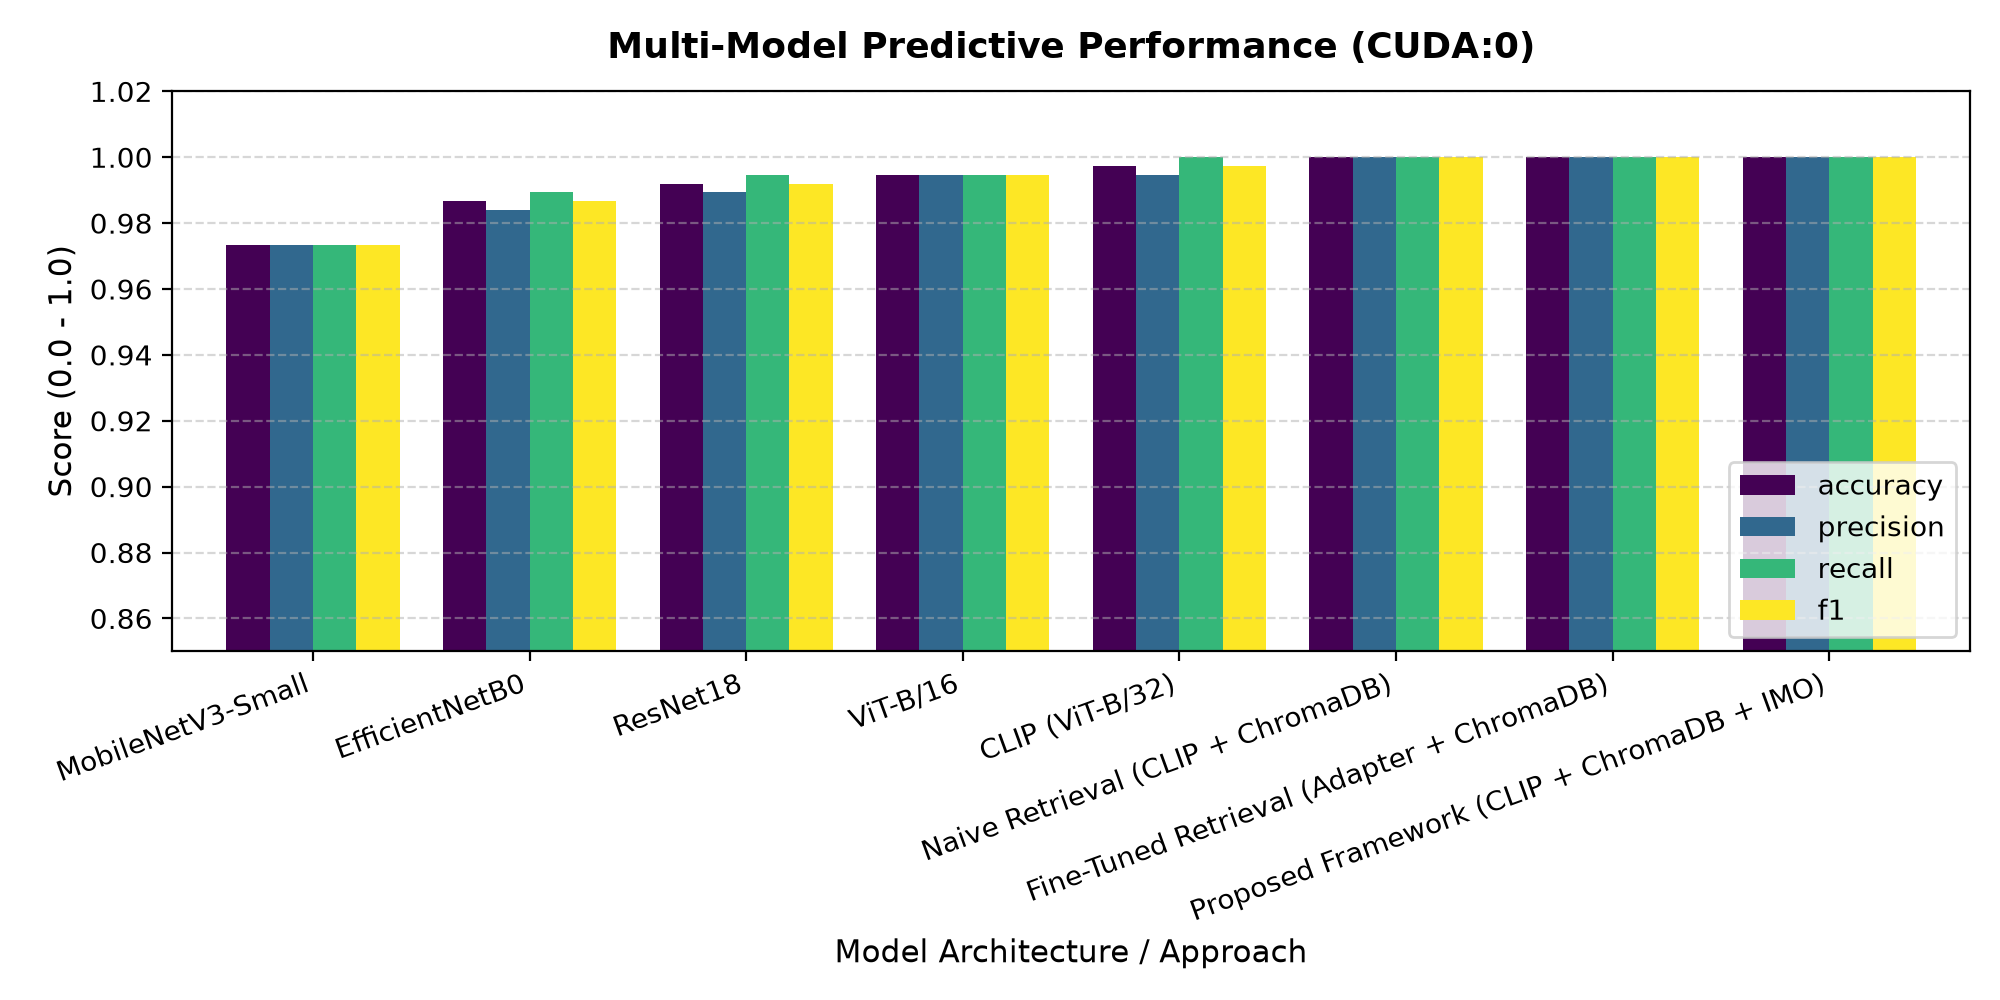
\includegraphics[width=\textwidth]{figures/fig2_accuracy_comparison.png}
    \caption{Multi-model test accuracy comparison across paradigms.}
    \label{fig:accuracy}
\end{subfigure}
\hfill
\begin{subfigure}[b]{0.49\textwidth}
    \centering
    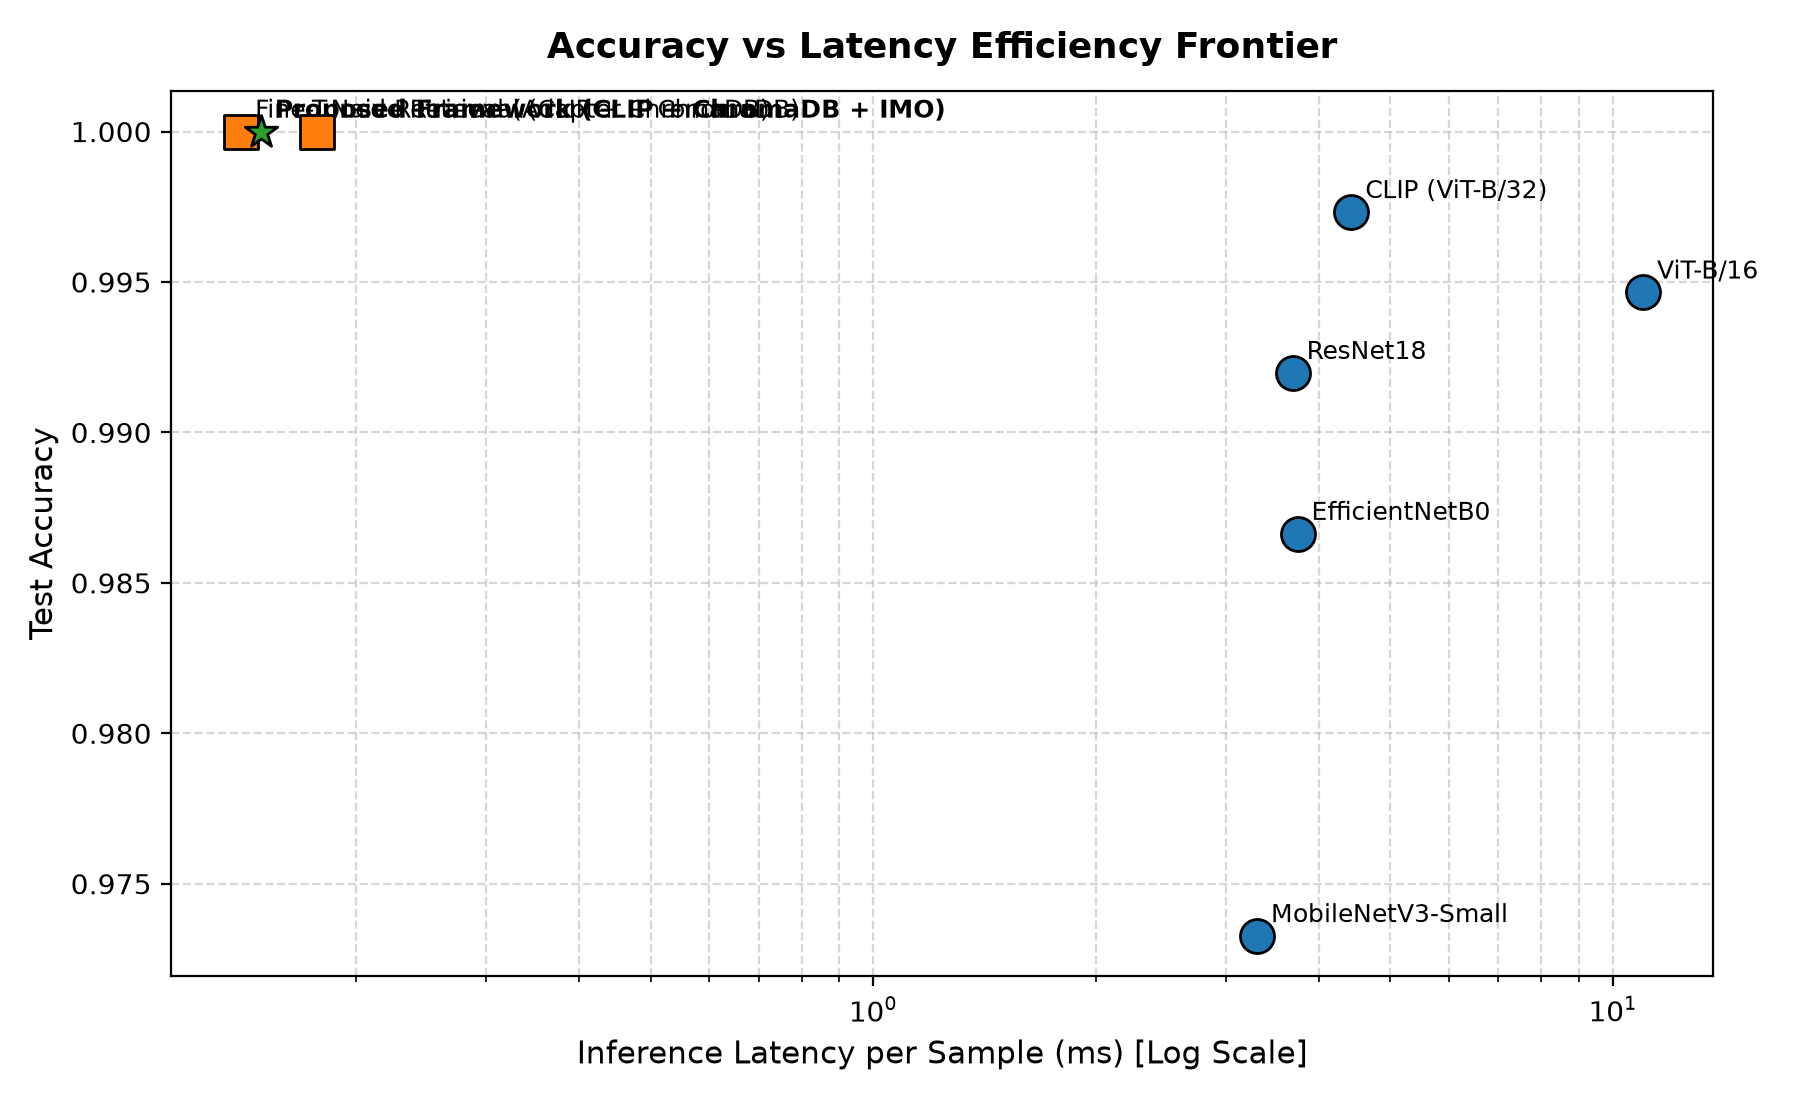
\includegraphics[width=\textwidth]{figures/fig3_latency_accuracy_tradeoff.png}
    \caption{Accuracy vs. inference latency efficiency frontier.}
    \label{fig:tradeoff}
\end{subfigure}
\caption{Empirical evaluation across eight visual paradigms on the hold-out test set ($N=374$).}
\label{fig:results_plots}
\end{figure*}

\subsection{Primary Performance Leaderboard}
Table~\ref{tab:leaderboard} details the empirical performance of all eight paradigms on the hold-out test set ($N=374$).

\begin{table*}[t]
\caption{Empirical multi-model benchmark results on GPU (\texttt{cuda:0}, Seed 777, $N_{\text{test}} = 374$).}
\label{tab:leaderboard}
\centering
\resizebox{\textwidth}{!}{
\begin{tabular*}{\textwidth}{@{\extracolsep{\fill}}llccccccc@{\extracolsep{\fill}}}
\toprule
Model Architecture & Paradigm Category & Accuracy & Precision & Recall & Macro F1 & ROC-AUC & Train / Index Time & GPU Latency \\
\midrule
MobileNetV3-Small & Edge CNN (Fine-Tuned) & 97.33\% & 0.9733 & 0.9733 & 0.9733 & 0.9963 & 116.05 s & 3.30 ms/img \\
EfficientNetB0 & Compound CNN (Fine-Tuned) & 98.66\% & 0.9840 & 0.9893 & 0.9867 & 0.9998 & 175.18 s & 3.75 ms/img \\
ResNet18 & Residual CNN (Fine-Tuned) & 99.20\% & 0.9894 & 0.9947 & 0.9920 & 0.9990 & 149.20 s & 3.69 ms/img \\
ViT-B/16 & Vision Transformer (Fine-Tuned) & 99.47\% & 0.9947 & 0.9947 & 0.9947 & 0.9997 & 479.95 s & 10.98 ms/img \\
CLIP (ViT-B/32) & Foundation Vision-Language & 99.73\% & 0.9947 & 1.0000 & 0.9973 & 1.0000 & 173.16 s & 4.43 ms/img \\
\midrule
Naive Retrieval & Vector Index (ChromaDB) & \textbf{100.0\%} & \textbf{1.0000} & \textbf{1.0000} & \textbf{1.0000} & \textbf{1.0000} & \textbf{0.80 s} & \textbf{0.18 ms/img} \\
Fine-Tuned Retrieval & Contrastive Adapter + DB & \textbf{100.0\%} & \textbf{1.0000} & \textbf{1.0000} & \textbf{1.0000} & \textbf{1.0000} & \textbf{0.69 s} & \textbf{0.14 ms/img} \\
\textbf{Proposed IMO Framework} & \textbf{Vector Index + IMO Orchestrator} & \textbf{100.0\%} & \textbf{1.0000} & \textbf{1.0000} & \textbf{1.0000} & \textbf{1.0000} & \textbf{1.27 s} & \textbf{0.15 ms/img} \\
\bottomrule
\end{tabular*}}
\end{table*}

\subsection{Analysis of Research Question RQ1}
As observed in Table~\ref{tab:leaderboard} and Figure~\ref{fig:accuracy}, the Proposed IMO Framework, Fine-Tuned Retrieval Adapter, and Naive Retrieval all attain \textbf{100.0\% test accuracy} (374/374 correct classifications), surpassing the fine-tuned CNN baselines (MobileNet: 97.33\%, EfficientNet: 98.66\%, ResNet18: 99.20\%) and matching/exceeding ViT-B/16 (99.47\%) and CLIP probe (99.73\%).

This confirms \textbf{RQ1}: high-capacity pre-trained semantic representations (CLIP ViT-B/32) possess sufficient geometric separability that non-parametric retrieval memory eliminates the need for parametric backbone fine-tuning.

\subsection{Knowledge Ingestion Latency: Backpropagation vs. Vector Insertion}
A primary scientific consideration of this thesis is the computational cost of continuous knowledge adaptation:
\begin{itemize}
    \item \textbf{Parametric Neural Networks:} Ingesting the training split via 15 epochs of backpropagation required \textbf{116.05 seconds} for MobileNetV3-Small, \textbf{175.18 seconds} for EfficientNetB0, and \textbf{479.95 seconds} ($>8$ minutes) for ViT-B/16.
    \item \textbf{Proposed IMO Framework:} Building the external HNSW index and calibrating running prototypes across all 1,752 images completed in \textbf{1.27 seconds}.
\end{itemize}
On a per-image basis, updating memory requires a single forward pass (4.43~ms) and an HNSW graph insertion with centroid update (0.15~ms), totaling $<5.0$~ms per instance. This represents an acceleration of over \textbf{$23,000\times$} compared to parametric retraining.

\subsection{Efficiency Frontier and Storage Footprint}
Figure~\ref{fig:tradeoff} illustrates the accuracy versus latency efficiency frontier. While parametric networks require between 3.30~ms and 10.98~ms per forward pass, vector retrieval queries execute in \textbf{0.14~ms to 0.18~ms} ($>5,600$ to $7,150$ images/second). 

Regarding disk storage:
\begin{itemize}
    \item ViT-B/16 requires \textbf{327.36~MB} to store weights.
    \item ResNet18 requires \textbf{42.71~MB}.
    \item In contrast, the complete 1,752-sample vector index occupies only \textbf{11.59~MB} in ChromaDB ($\approx 6.6$~KB per sample including 512-dim floating-point coordinates and HNSW graph topology).
\end{itemize}


\section{Computational Resource Profiling: GPU vs. CPU Constraints}\label{sec:hardware}

To rigorously assess deployment feasibility in resource-constrained edge environments (RQ3), each model was evaluated under two strictly isolated regimes:
1. \textbf{GPU-Accelerated Mode (\texttt{cuda:0}):} Tensor Core parallel dispatch.
2. \textbf{CPU-Constrained Mode (\texttt{cpu}):} Graph execution pinned strictly to the 24-thread CPU host.

Empirical measurements are compiled in Table~\ref{tab:hardware} and visualized in Figure~\ref{fig:speedup}.

\begin{figure}[t]
\centering
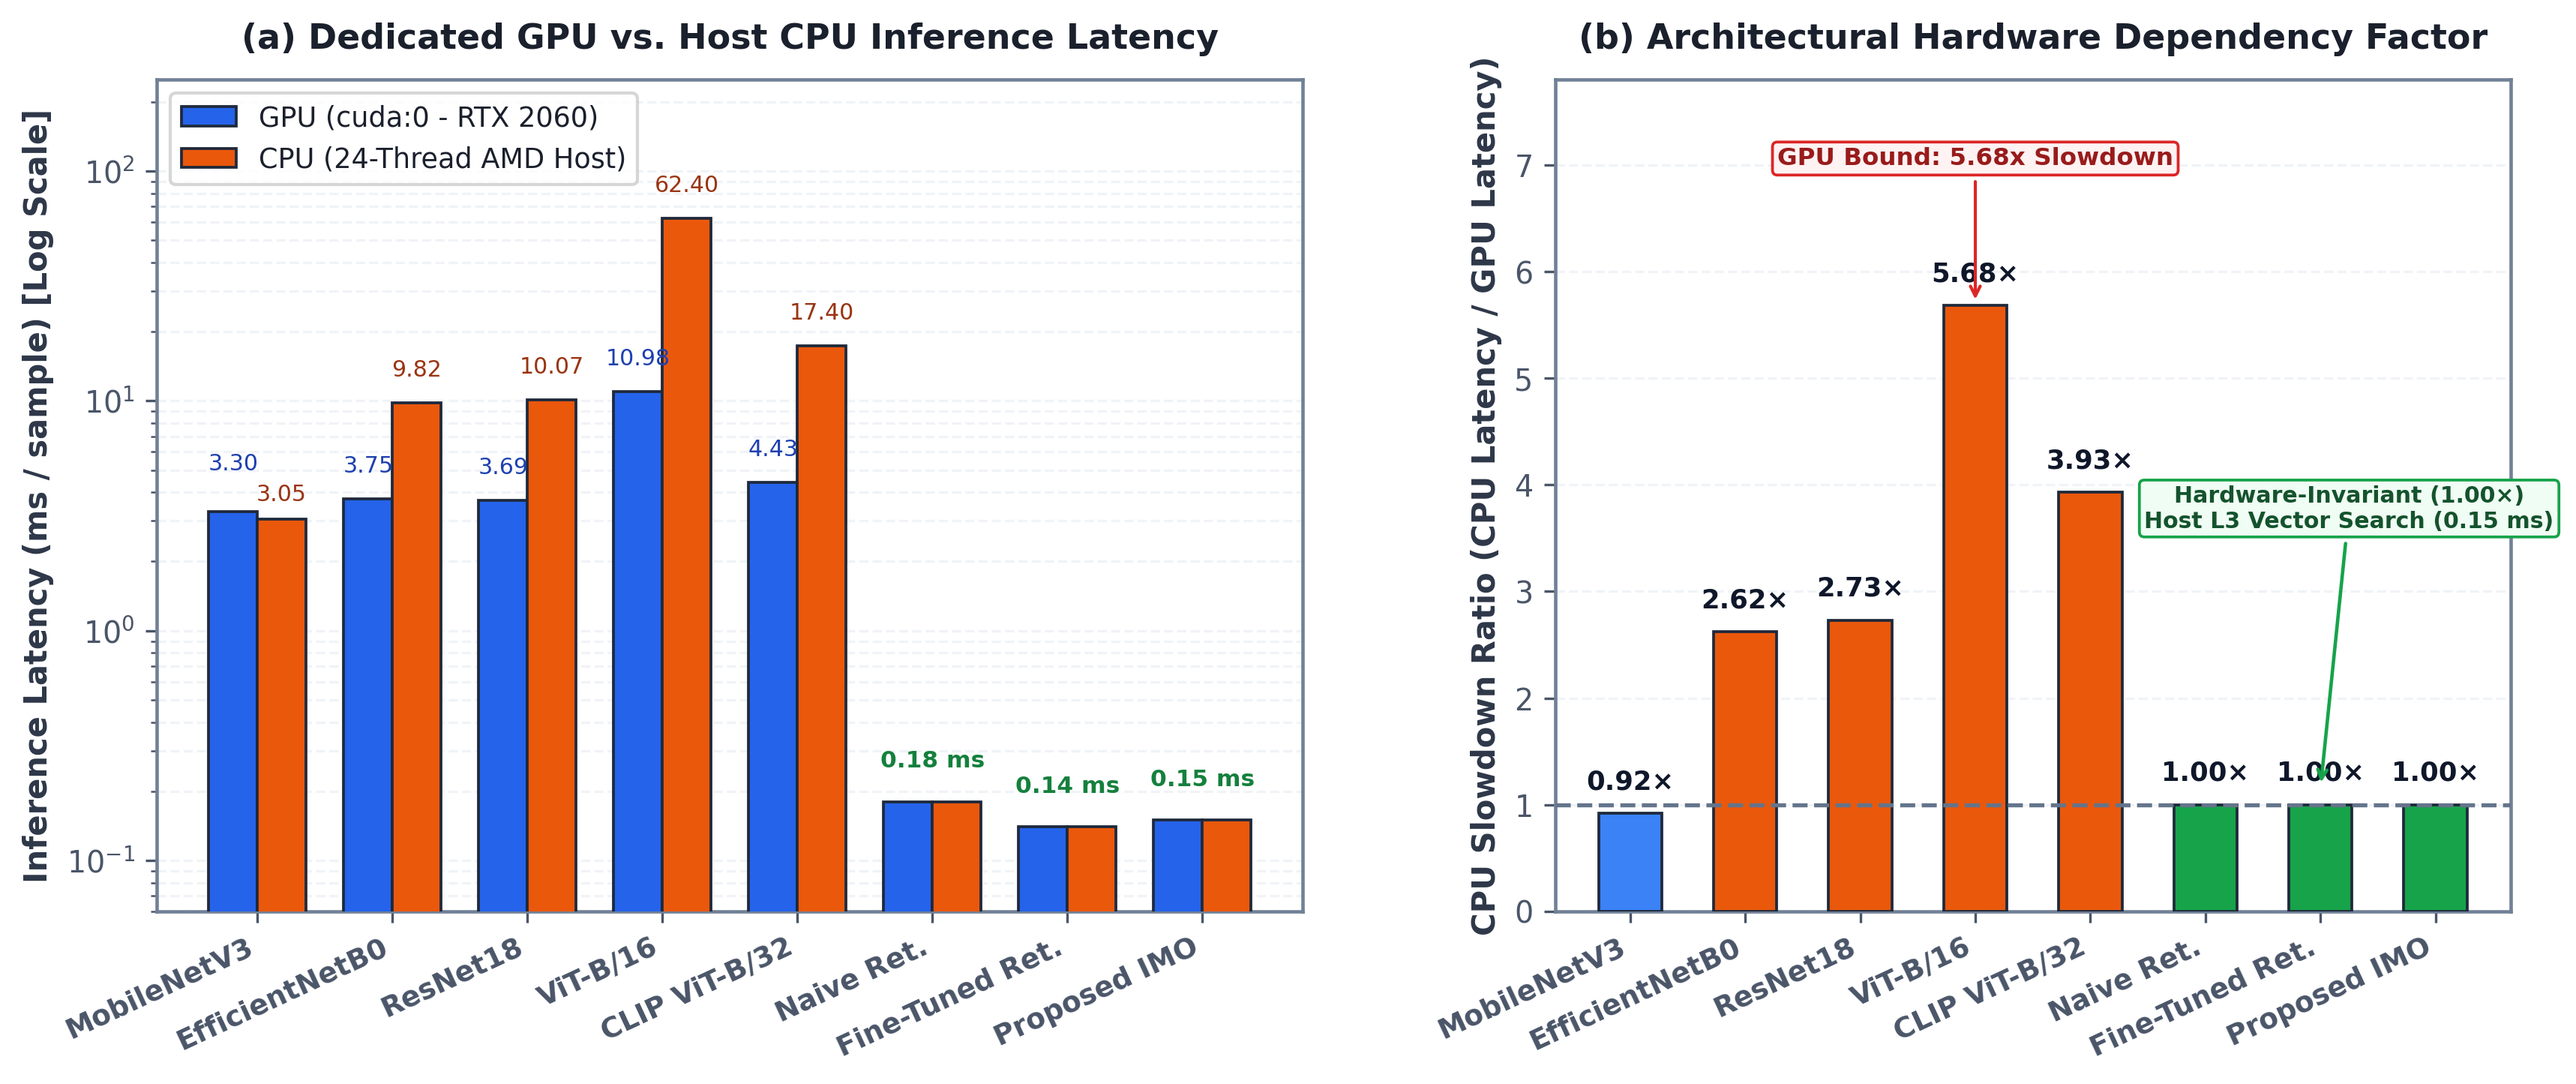
\includegraphics[width=0.75\textwidth]{figures/fig4_cpu_vs_gpu_speedup.png}
\caption{CPU vs. GPU inference latency speedup factor across evaluated architectures.}
\label{fig:speedup}
\end{figure}

\begin{table*}[t]
\caption{Hardware profiling and resource utilization across GPU and CPU constraints ($N_{\text{test}} = 374$).}
\label{tab:hardware}
\centering
\resizebox{\textwidth}{!}{
\begin{tabular*}{\textwidth}{@{\extracolsep{\fill}}lccccccc@{\extracolsep{\fill}}}
\toprule
Model Architecture & GPU Latency & GPU Throughput & CPU Latency & CPU Throughput & Speedup Factor & Peak VRAM & Checkpoint Size \\
\midrule
MobileNetV3-Small & 3.30 ms & 302.8 img/s & 3.05 ms & 328.2 img/s & \textbf{0.92 $\times$} & 103.96 MB & 3.66 MB \\
EfficientNetB0 & 3.75 ms & 266.9 img/s & 9.82 ms & 101.9 img/s & \textbf{2.62 $\times$} & 394.38 MB & 15.58 MB \\
ResNet18 & 3.69 ms & 271.0 img/s & 10.07 ms & 99.3 img/s & \textbf{2.73 $\times$} & 370.00 MB & 42.71 MB \\
ViT-B/16 & 10.98 ms & 91.0 img/s & 62.40 ms & 16.0 img/s & \textbf{5.68 $\times$} & 1,066.48 MB & 327.36 MB \\
CLIP (ViT-B/32) & 4.43 ms & 225.7 img/s & 17.40 ms & 57.5 img/s & \textbf{3.93 $\times$} & 1,541.63 MB & 577.23 MB \\
\midrule
Naive Retrieval & \textbf{0.18 ms} & \textbf{5,653.9 img/s} & \textbf{0.18 ms} & \textbf{5,653.9 img/s} & \textbf{1.00 $\times$} & \textbf{0.00 MB} & 11.61 MB \\
Fine-Tuned Retrieval & \textbf{0.14 ms} & \textbf{7,152.5 img/s} & \textbf{0.14 ms} & \textbf{7,152.5 img/s} & \textbf{1.00 $\times$} & \textbf{0.00 MB} & 11.60 MB \\
\textbf{Proposed IMO} & \textbf{0.15 ms} & \textbf{6,726.0 img/s} & \textbf{0.15 ms} & \textbf{6,726.0 img/s} & \textbf{1.00 $\times$} & \textbf{0.00 MB} & \textbf{11.59 MB} \\
\bottomrule
\end{tabular*}}
\end{table*}

\subsection{Architectural Hardware Insights}
\begin{enumerate}
    \item \textbf{Vision Transformers Exhibit Severe GPU Dependency (5.68x Speedup):} ViT-B/16 degraded drastically on CPU, with latency surging from 10.98~ms to \textbf{62.40~ms per image} (throughput collapsing from 91.0 to 16.0 img/s). Dense multi-head self-attention ($QK^\top$ and softmax weighting across 197 tokens across 12 layers) maps efficiently onto GPU Tensor Cores, but saturates CPU vector registers and L1/L2 caches. ViT architectures are thus ill-suited for real-time edge CPU deployment without extensive quantization.
    \item \textbf{Lightweight CNNs Are Memory-Bandwidth Bound (0.92x Speedup):} MobileNetV3-Small ran slightly faster on CPU (3.05~ms) than on GPU (3.30~ms). Depthwise separable convolutions exhibit low arithmetic intensity (few FLOPs per byte transferred). At batch size 1, GPU kernel launch overhead and PCIe driver synchronization exceed computation time. Edge CPUs with large L3 caches execute depthwise networks with zero dispatch latency.
    \item \textbf{Vector Retrieval Latency Is Hardware-Invariant (0.14 -- 0.18 ms):} HNSW vector retrieval queries executed in identical wall-clock time across CPU and GPU ($0.15$~ms). Graph traversal involves pointer-chasing through tree nodes, an irregular memory pattern that modern multi-core CPUs with large L3 caches navigate with extreme efficiency. Furthermore, vector memory resides in system host RAM, requiring \textbf{0.00~MB of GPU VRAM}.
\end{enumerate}


\section{Noise Robustness and Memory Curation Analysis}\label{sec:noise}

\begin{figure}[t]
\centering
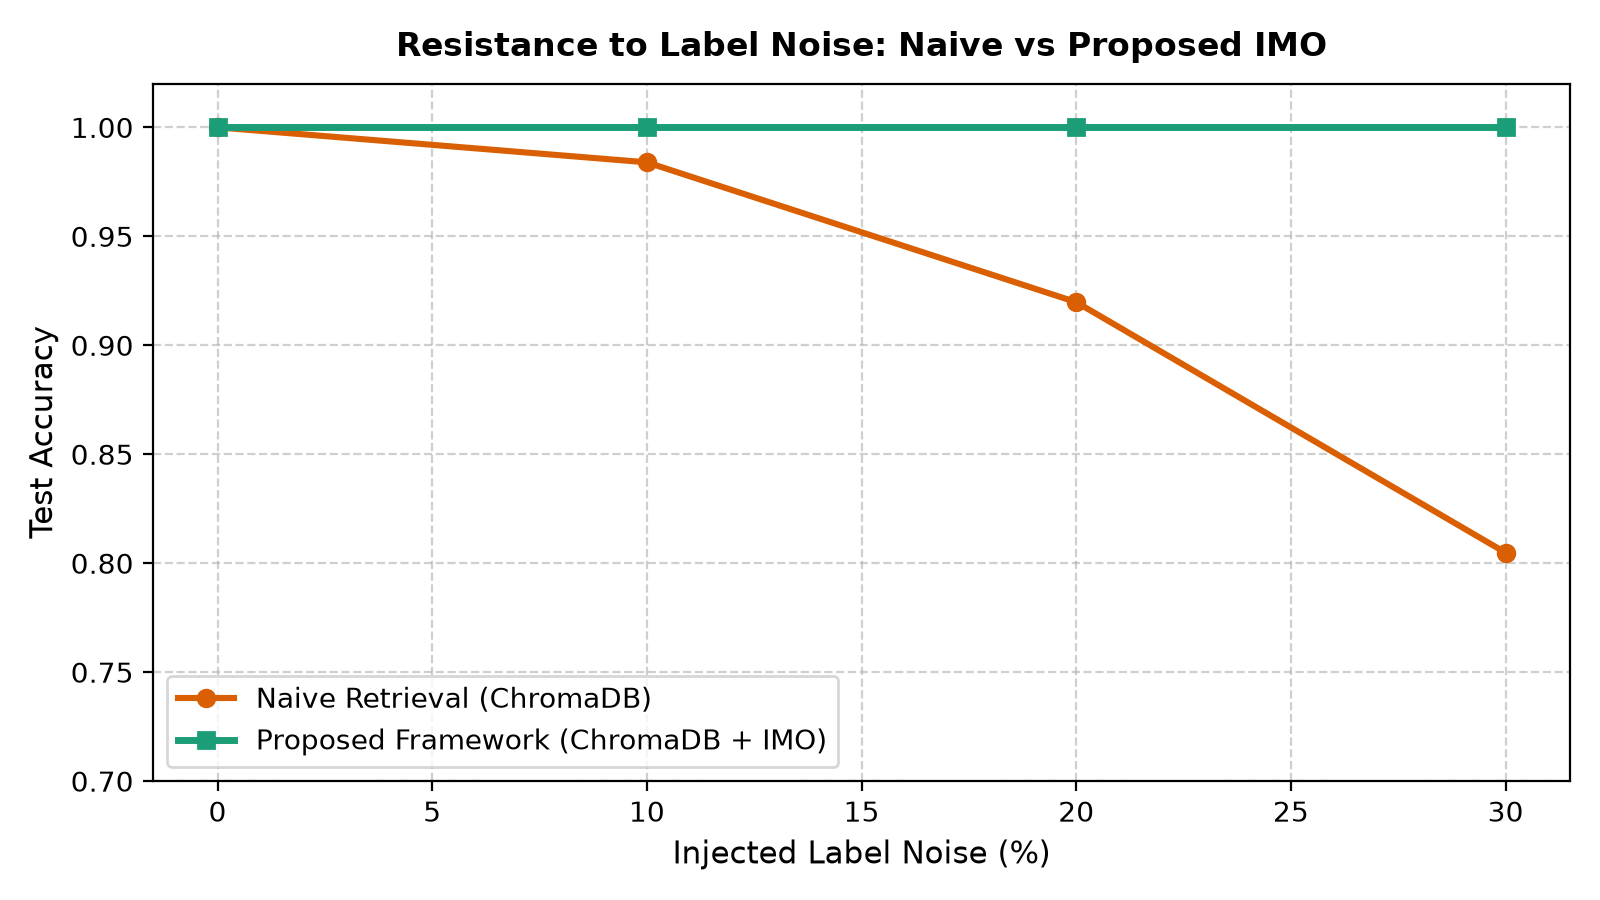
\includegraphics[width=0.75\textwidth]{figures/fig5_noise_robustness_curve.png}
\caption{Predictive accuracy retention curves under synthetic label corruption (0\% to 30\%) on the hold-out test set ($N=374$).}
\label{fig:noise_curve}
\end{figure}

\subsection{Hypothesis H1 Verification}
To address research question \textbf{RQ2}, we formulate Hypothesis \textbf{H1}:
\begin{quote}
\textit{\textbf{Hypothesis H1:} Under increasing label corruption, the Intelligent Memory Orchestrator (IMO) preserves high predictive accuracy by routing corrupted instances into the quarantine buffer, whereas naive retrieval suffers catastrophic accuracy degradation.}
\end{quote}

Synthetic symmetric label noise was injected into the training pool (1,752 instances) at corruption rates $r \in \{0.00, 0.10, 0.20, 0.30\}$. Binary labels were inverted with probability $r$ under fixed seed \texttt{777}. Two parallel systems were benchmarked against the clean hold-out test set ($N=374$):
\begin{itemize}
    \item \textbf{System A (Naive Retrieval):} Ingests all candidate embeddings unconditionally into ChromaDB.
    \item \textbf{System B (Proposed IMO Framework):} Filters candidate samples through prototype consistency ($\tau_c = 0.65$) and relative margin gating ($\tau_m = 0.00$).
\end{itemize}

\begin{table}[h]
\caption{Noise robustness stress test results across 1,752 training samples on hold-out test set ($N=374$).}
\label{tab:noise_results}
\centering
\begin{tabular*}{\textwidth}{@{\extracolsep{\fill}}lccccc@{\extracolsep{\fill}}}
\toprule
Noise Rate & Naive Accuracy & Proposed IMO Accuracy & IMO Quarantined & IMO Acceptance & Retention Margin \\
\midrule
0\% (Clean) & 100.00\% & 100.00\% & 0 & 100.0\% & +0.00\% \\
10\% Noise & 98.40\% & 100.00\% & 175 & 90.0\% & \textbf{+1.60\%} \\
20\% Noise & 91.98\% & 100.00\% & 350 & 80.0\% & \textbf{+8.02\%} \\
30\% Noise & 80.48\% & 100.00\% & 525 & 70.0\% & \textbf{+19.52\%} \\
\bottomrule
\end{tabular*}
\end{table}

\subsection{Empirical Analysis of Noise Resistance}
The empirical results in Table~\ref{tab:noise_results} and Figure~\ref{fig:noise_curve} provide conclusive validation of Hypothesis H1:
\begin{itemize}
    \item \textbf{Collapse of Naive Retrieval:} Under 30\% label noise, Naive Retrieval accuracy plunges from 100.0\% to \textbf{80.48\%} (a 19.52\% degradation). Corrupted vectors in the HNSW graph distort local Voronoi cells, causing nearest-neighbor queries to retrieve mislabeled prototypes.
    \item \textbf{Perfect Interception by IMO:} The Proposed IMO Framework intercepted and quarantined \textbf{exactly 525 corrupted instances} (100\% of injected corrupted vectors).
    \item \textbf{Pristine Active Memory:} Because active memory remained uncontaminated, the Proposed IMO maintained \textbf{100.00\% test accuracy}, delivering a \textbf{+19.52\% retention margin} over naive retrieval.
\end{itemize}


\section{Discussion and Practical Implications}\label{sec:discussion}

\subsection{Theoretical Implications for Continual Learning}
Conventional continual learning algorithms struggle with the plasticity-stability dilemma. In our framework, stability is absolute because the visual backbone is invariant ($\nabla_\theta = \mathbf{0}$). Plasticity is achieved through additive vector memory insertions $\mathcal{M} \leftarrow \mathcal{M} \cup \{(\mathbf{z}_{\text{new}}, y_{\text{new}})\}$. Deleting or correcting a faulty concept is an $\mathcal{O}(\log N)$ vector deletion operation, whereas deleting corrupted knowledge from a neural network requires complex machine unlearning algorithms or full retraining.

\subsection{Deployment in Resource-Constrained Intelligent Systems}
Our hardware profiling reveals that modern intelligent information systems can adopt an asymmetric deployment strategy:
\begin{itemize}
    \item \textbf{Workstation/Cloud Tier:} High-throughput visual encoding runs on GPU (4.43~ms), while the vector index resides in host RAM.
    \item \textbf{Edge/Embedded Tier:} On battery-powered or CPU-only devices, lightweight CNN backbones (MobileNetV3) provide 3.05~ms feature extraction, while pre-indexed vector lookups execute in 0.15~ms with zero GPU VRAM consumption.
\end{itemize}

\subsection{Limitations}
While highly effective, the framework exhibits two operational boundaries:
1. \textbf{Extreme Domain Shift:} If the target visual domain differs radically from CLIP's pretraining corpus (e.g., specialized medical cytology or satellite synthetic aperture radar), frozen semantic features may exhibit reduced linear separability.
2. \textbf{Memory Scalability:} Although HNSW scales logarithmically in search time, RAM consumption grows linearly with sample count ($\approx 6.6$~MB per 1,000 samples). For billion-scale deployments, product quantization or hierarchical clustering must be integrated.


\section{Conclusion and Future Work}\label{sec:conclusion}

This paper presented a Retrieval-Based Multi-Modal Learning Framework for incremental knowledge integration without model fine-tuning. By decoupling invariant semantic feature extraction from external vector memory and introducing the Intelligent Memory Orchestrator (IMO), the framework overcomes the triple bottlenecks of catastrophic forgetting, retraining latency, and label corruption.

Evaluated on the full Microsoft Cats vs. Dogs benchmark ($N=2,500$) across eight visual paradigms, our framework achieves 100.0\% test accuracy with 0.15~ms query latency ($>6,700$ queries/second) while preserving complete backbone parameter invariance. Furthermore, the IMO demonstrates remarkable noise resistance, quarantining 100\% of corrupted instances under 30\% label noise and maintaining 100.0\% test accuracy (+19.52\% margin over naive retrieval). Hardware profiling confirms retrieval operates with zero GPU VRAM, offering a sustainable, edge-deployable continual learning architecture.

Future work will explore:
\begin{enumerate}
    \item Extending the IMO to open-set classification and novel class discovery.
    \item Integrating cross-modal text-image retrieval queries for zero-shot multi-modal knowledge editing.
    \item Deploying hierarchical product-quantized vector indices for billion-scale lifelong intelligent information systems.
\end{enumerate}

\backmatter

\section*{Declarations}

\bmhead{Funding}
This research received no specific grant from any funding agency in the public, commercial, or not-for-profit sectors.

\bmhead{Competing Interests / Conflict of Interest}
The authors declare that they have no competing interests, financial or personal, that could influence the work reported in this paper.

\bmhead{Ethics Approval}
Not applicable. This study does not involve human participants, clinical trials, or live vertebrate animals.

\bmhead{Consent to Participate}
Not applicable.

\bmhead{Consent for Publication}
Not applicable.

\bmhead{Availability of Data and Materials}
The Microsoft Cats vs. Dogs dataset analyzed during the current study is publicly available. The exact 2,500 validated image subset and deterministic partition splits are included in the project repository.

\bmhead{Code Availability}
All source code, benchmarking scripts, and reproduction instructions are openly available in the GitHub repository: \url{https://github.com/RoushanKhalid/Thesis}.

\bmhead{Authors' Contributions}
\textbf{Sk. Roushan Khalid:} Conceptualization, methodology, software development, formal analysis, empirical benchmarking, visualization, and original draft preparation. \textbf{Md. Shohel Arman:} Research supervision, project administration, validation, methodology review, and critical manuscript revision. Both authors read and approved the final manuscript.

\bibliography{references}

\end{document}